\documentclass[12pt,a4paper]{article}
\usepackage[utf8]{inputenc}
\usepackage{amsmath}
\usepackage{amsfonts}
\usepackage{amssymb}
\usepackage{color}
\usepackage{listings}
\author{K.M.J. Jacobs (s4134621) \and Zhuoran Liu (s4594851) \and Ankur Ankan (s4753828) \and Code file: MNIST.ipynb}
\title{Multi-Layer Perceptron}
\usepackage{graphicx}

\begin{document}
\maketitle

\color{black}
\newpage
\section{Introduction}
In this report, we will consider the neural network multi-layer perceptron. Multi-layer perceptron is a neural network with multiple hidden layers and in each hidden layer there are multiple neurons. Between different neurons in adjacent layers, there exist weights to connect different neurons. In every hidden layer, there exist biases to tune some outcomes of neurons. The aim of training the network is to find the proper weights and biases which can be used to predict the new data.
\subsection{Underlying Theory}
The working mechanism of the MLP is like following. Given the neural network structure(weights matrix $W$ and biases vector $b$) and input data vector $a$, we can calculate the feed forward process by formula
\[\textbf{z} = g(\textbf{w}a + \textbf{b})\]
Here $g$ is the activation function and output $z$ is a vector. Use $z$ as the input of the next layer, we can do similar calculation again until we get the output. Given the last output $z$, we will calculate the $argmax(z)$. The category of the $argmax(z)$ is the predication of the input $a$. Given the right category(training targets), we can tune the weights and biases to predict better and better. This is the learning process of MLP. 
\subsection{Learning Algorithm}
Backpropagation algorithm is the learning algorithm we will use. It consists of 4 steps.
\[\delta^L = \nabla_{a} C \circ \sigma'(z^{L})\]
\[\delta^L = ((w^{l+1})^{T} \delta^{l+1} \circ \sigma'(z^{l})\]
\[\frac{\partial C}{\partial b_{j}^{l}} = \sigma_{j}^{l}\]
\[\frac{\partial C}{\partial w_{jk}^{l}} = a_{k}^{l-1} \sigma_{j}^{l}\]
Here symbol $\circ$ means Hadamard product.$a_k^l$ means neuron $k$ in the $l$th layer.\\
These four step will backpropagate error and output the gradient change of cost function. The whole process is input, feedforward, backpropagate, update weights and biases, input again... Finally after many epoches we will get the final neural network with particular weights and biases, then we finish training.
\newpage
\section{Problem statement}
1. The influence of different number of layers and different number of neurons.\\
2. The different influences of defferent initializations of the weights and biases before learning.\\
3. Influences by choosing different activation functions.\\
4. Compare two different learning method - Stochastic Gradient Descent vs. Momentum.\\

\section{Results}
\subsection{The structure of Multi-Layer Perceptron}
\subsubsection{Different neurons}
The first problem to investigate is the influence on classification accuracies from the number of neurons in hidden layers. We did the experiment with five different settings. All the settings have one hidden layer with different neurons. All five experiments used same input layer ($784$) and output layer, and used same epoches (1$50$), same learning rate ($0.05$) and same mini-batch number ($10$). Figure 1. shows the results of five different setting.Blue line is $2$ neurons, red line is $5$ neurons, black line is $10$ neurons, green line is $20$ neurons and magenta line is $100$ neurons.\\
\begin{figure}
\centering
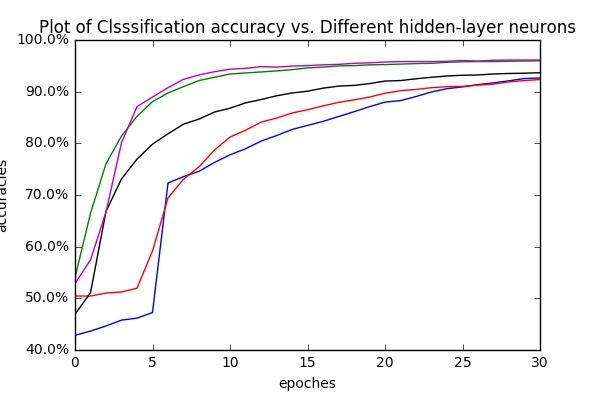
\includegraphics[width=60mm,scale=1]{p106.jpg}
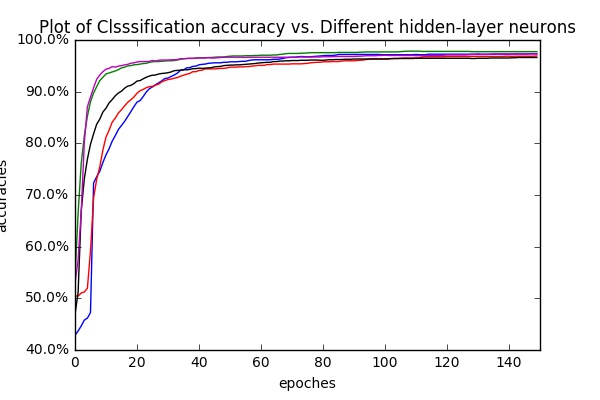
\includegraphics[width=60mm,scale=1]{p101.jpg}
\caption{Different learning processess by different setting of neuron number with one hidden layer}
\end{figure}\\
In figure 1, the horizontal axis showed the epoches changed from $0$ to $150$, and the vertical axis showed the test accuracies in percentage. The formula used here is
\[\text{accuracy} = \frac{\text{right classified number in test images}}{ \text{total number in test images}}\]\\

From the left plot we can easily see that, if there is one hidden layer, more hidden neurons will yield better results in small number of epoches.For example, the magenta line($100$ neurons) did better than others before $30$ epoches. \\
But from right side plot, by large amount of epches, intermediate number of neurons had better results. For example, green line ($20$ neurons) is better than others in right side plot.\\
Here the possible reason is over-fitting, since more neurons will yield more complex model. After training many steps, the model is too complex. So had a worse accuracies on test set.\\

\begin{figure}
\centering
\includegraphics[width=90mm,scale=1]{p102.jpg}\\
\caption{Different learning time by different setting of neuron number with one hidden layer}
\end{figure}

We also need to consider the running time of different cases. In figure 2, it is obvious that more neurons will take more training time, and the relationship between neurons' number and time cost is almost linear. Since we used only one layer, it will just have more calculations by neurons. So it is reasonable here.\\
\subsubsection{Different layers}
The second problem to investigate is the influence on classification accuracies from the number of hidden layers. We did the experiment with five different settings. The settings of hidden layer number ranges from $1$ to $5$, and in each hidden layer we used $5$ neurons. All five experiments used same input layer ($784$) and output layer, and used same epoches ($100$), same learning rate ($0.05$) and same mini-batch number ($10$). The figure 3 and figure 4 showed the results of five different settings.\\
\begin{figure}
\centering
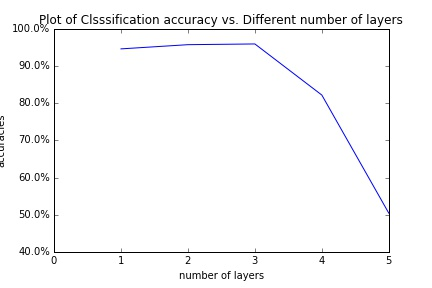
\includegraphics[width=90mm,scale=1]{p103.jpg}
\caption{Different learning accuracies by different setting of layer numbers}
\end{figure}

\begin{figure}
\centering
\includegraphics[width=90mm,scale=1]{p104.jpg}
\caption{Different learning time by different setting of layer numbers}
\end{figure}

From figure 3, we can see that more hidden layers had a bad performance after layers' amout $3$. It increased a little bit from layer number $1$ to $3$, then dropped after $3$.\\
The other experiments almost performed much better This problem may be caused by the training data. Since we just need to classify number $3$ and number $7$, so no more complicated model should be trained. So more layers didn't perform better. But this is no the general case.\\


More layers will take more training time, and the relationship between layers' number and time is also almost linear. The figure 4 is the running time of the five experiments we mentioned above. This relationship may not be the same, when we have more neurons in every layer and when we have more layers. It will be like exponential time, but not really. Since all the calculations are linear.\\

\subsection{The initialization of the weights and biases}
By default we choose the initialization of weights and biases using Gausssian random variables with mean $0$ and deviation $1$. Here we used another way to improve it such that we can have a better initialization and better results.

We mainly considered the initialization with a normalized Gaussian. The formula is\\
\[\text{initialization of weights}= \frac{\text{random} (y, x)}{\sqrt{x}}\]\\
This setting can make the distribution more sharply peaked which makes it less likely that neuron will saturate. We did experiment for both initializations and have the results below.Both experiments used same input layer ($784$) and output layer, and used same epoches ($150$), same learning rate ($0.05$) and same mini-batch number ($10$).Both with $1$ hidden layer and $100$ neurons. The plot below shows the results of two different settings.\\
\subsubsection{different initialization of weights and biases}
\begin{figure}
\centering
\includegraphics[width=90mm,scale=1]{p201.jpg}
\caption{Different initializations of weights and biases}
\end{figure}
From the figure 5, we can easily see that. Optimized initialization with a normalizing component will make the initial accuracy munch higher than the default gaussian distribution. Also it showed a better result than the default setting. Since the distribution is more sharply peaked, it less likely that neuron will saturate.
\subsubsection{different activation functions}
By default we used sigmoid function as the activation function. Here we compared the sigmoid function with tanh function.\\
\begin{figure}
\centering
\includegraphics[width=60mm,scale=1]{p301.jpg}
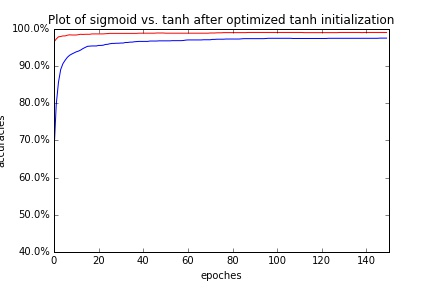
\includegraphics[width=60mm,scale=1]{p302.jpg}
\caption{Different activation functions in same structure}
\end{figure}
From figure 6 left side, we can see that sigmoid did better. Here should not be so much difference, so we optimized the initialization of tanh function. The result is on the right side plot. It showed that tanh activation function did the process better. We can conclude that different activations functions have different performances, and it really depended on the initializations of weights and biases. Because at initialization we want the weights to be small enough around the origin so that the activation function operates in its linear regime, where gradients are the largest.

\subsection{Different learning methods}
\subsubsection{Stochastic gradient descent vs. Momentum}
Momentum is a method to escape from local minimum, and it did speed up the learning process by changing gradient direction more straight forward to the target. We used two formulas to implement the momentum learning.
\[v' = \mu v - \eta \nabla C\]
\[w' = w + v'\]
After implementation we got the results compared with stochastic gradient method as below. In figure 7, red line showed the process of stochastic gradient descent and blue line showed the process of momentum. The momentum convergence faster than SGD. Since it changed more in every step than SGD, it fluctuated a little bit. From this figure it is not very obvious, but momentum method is more stable than SGD.\\
\begin{figure}
\centering
\includegraphics[width=75mm,scale=1]{p401.jpg}\\
\end{figure}

\section{Discussion and Conclusion}
Multi-layer perceptron is perceptron which can be trained by various patterns. It is not easy to be trained well. This training process depended on many aspects. For example number of neurons, number of layers, initialization of weights and biases, learning methods, learning rates, size of mini-batches and so on. \\

From what we have explored, more hidden layers and more neurons involved may have better results, but it will also take more time and cause over-fitting. The time has a similar linear relationship with the number of neurons and the number of hidden layers. A good initialization can obviously improve the initial accuracy of the learning process, and it also help tune the weights and biases better. Different activation functions have different influences on the accuracies of test, and they have also different running time. The choose of learning rate, epoches and mini batch sizes are also import parts. But they can be investigated by some experiments and choose the comparable better one.

\newpage
\section{Appendix}
\subsection{Load, reshape and transform the raw data to training set with $3$ and $7$}
\begin{lstlisting}[language=Python]
import numpy as np
np.set_printoptions(threshold=np.nan)
import scipy.io
import scipy
import random


class DataLoader:
    '''
    For load data and change shape to (x,y). x is the traing images and y is the label of the x.
    '''

    def __init__(self, file):

        self.data = scipy.io.loadmat(file, squeeze_me=True, struct_as_record=False)['mnist']
        self.train_images = self.data.train_images
        self.test_images = self.data.test_images
        self.train_labels = self.data.train_labels
        self.test_labels = self.data.test_labels

        # transform the raw data to binary data
        self.train_images = self.transform_images(self.train_images)
        self.test_images = self.transform_images(self.test_images)

        # reshape the training images to [784,1]
        self.train_images = [np.reshape(x, (784, 1)) for x in self.train_images]
        self.test_images = [np.reshape(x, (784, 1)) for x in self.test_images]

        labels = np.asarray(self.train_labels)
        selector = (labels == 3) | (labels == 7)
        self.train_labels = self.train_labels[selector]
        self.train_images = np.array(self.train_images)
        self.train_images = self.train_images[selector]
        ls= []
        for i in self.train_labels:
            if i == 3:
                ls.append([[1.],[0.]])
            else:
                ls.append([[0.],[1.]])
        self.train_labels = ls
        
        self.training_data = tuple(zip(self.train_images, self.train_labels))
        
#       test part
        labels = np.asarray(self.test_labels)
        selector = (labels == 3) | (labels == 7)
        self.test_labels = self.test_labels[selector]
        self.test_images = np.array(self.test_images)
        self.test_images = self.test_images[selector]
        ls= []
        for i in self.test_labels:
            if i == 3:
                ls.append([[1.],[0.]])
            else:
                ls.append([[0.],[1.]])
        self.test_labels = ls
        
        self.test_data = tuple(zip(self.test_images, self.test_labels))
        
        
    # function to reshape
    def transform_images(self, data):

        reshaped = data.reshape(data.shape[0] * data.shape[1], data.shape[2])
        swapped_axes = np.swapaxes(reshaped, 0, 1)
        return swapped_axes * (1.0/256)
#         return (swapped_axes > 122) * 2.0 - 1
\end{lstlisting}
\subsection{Main part of Network and Backpropagation}
\begin{lstlisting}[language=Python]
data = DataLoader('mnistALL.mat')
class Network(object):

    def __init__(self, sizes):
        '''
        sizes is the structure of the whole network shown by [first layer, second layer, ... , last year] as a list
        different waies to initialize the weights and biases
        '''
        self.num_layers = len(sizes)
        self.sizes = sizes
#       the initialization of the weights and biases
        self.biases = [np.random.randn(y, 1) for y in sizes[1:]]
        self.weights = [np.random.randn(y, x)
                        for x, y in zip(sizes[:-1], sizes[1:])]

    # the feedward calculation of the network, which will return the result to the last layer
    def feedforward(self, a):
        for b, w in zip(self.biases, self.weights):
            a = sigmoid(np.dot(w, a)+b)
        return a
    # stochastic gradient descent process, with training_data shaped like (x,y), x is the traing data,
#     and y is the target value. lr is the learning rate and mini_batch_size is mini batch size. test_data
#  is the part for validation
    def StochasticGradientDescent(self, training_data, epochs, mini_batch_size, lr,
            test_data=None):
        error = []
        if test_data: n_test = len(test_data)
        n = len(training_data)
        for j in xrange(epochs):
# shuffle command for shuffle the data set
            random.shuffle(list(training_data))
# here is the mini batches to train every time after shuffle the whole training set
            mini_batches = [
                training_data[k:k+mini_batch_size]
                for k in xrange(0, n, mini_batch_size)]
# here is to test the validation percentage of the model
            for mini_batch in mini_batches:
                self.update_mini_batch(mini_batch, lr)
            if test_data:
                error.append(self.evaluate(test_data)/(len(test_data) * 1.0))
                print "Epoch {0}: {1} / {2}".format(
                    j, self.evaluate(test_data), n_test)
                
            else:
                print "complete"
        return error
# this function is to update the weights and biases after mini batches
    def update_mini_batch(self, mini_batch, lr):
# initialization the nabla
        nabla_b = [np.zeros(b.shape) for b in self.biases]
        nabla_w = [np.zeros(w.shape) for w in self.weights]
        for x, y in mini_batch:
            delta_nabla_b, delta_nabla_w = self.backprop(x, y)
# here got updated by backpropagate
            nabla_b = [nb+dnb for nb, dnb in zip(nabla_b, delta_nabla_b)]
            nabla_w = [nw+dnw for nw, dnw in zip(nabla_w, delta_nabla_w)]
# did the update
        self.weights = [w-(lr/len(mini_batch))*nw
                        for w, nw in zip(self.weights, nabla_w)]
        self.biases = [b-(lr/len(mini_batch))*nb
                       for b, nb in zip(self.biases, nabla_b)]
# here is the specific backpropagate function
    def backprop(self, x, y):

        nabla_b = [np.zeros(b.shape) for b in self.biases]
        nabla_w = [np.zeros(w.shape) for w in self.weights]
        activation = x
        activations = [x] 
        zs = [] 
        # list to store all the z vectors, layer by layer
        for b, w in zip(self.biases, self.weights):
            z = np.dot(w, activation)+b
            zs.append(z)
#         here the activation function is sigmoid
            activation = sigmoid(z)
            activations.append(activation)
        # this is the delta back pass to update
        delta = self.cost_derivative(activations[-1], y) * \
            sigmoid_derive(zs[-1])
        nabla_b[-1] = delta
        nabla_w[-1] = np.dot(delta, activations[-2].transpose())
        
        for l in xrange(2, self.num_layers):
            z = zs[-l]
            sp = sigmoid_derive(z)
            delta = np.dot(self.weights[-l+1].transpose(), delta) * sp
            nabla_b[-l] = delta
            nabla_w[-l] = np.dot(delta, activations[-l-1].transpose())
#         got the final nablas for weights and biases
        return (nabla_b, nabla_w)
# here evaluate the whole correctness of the training samples
    def evaluate(self, test_data):
        test_results = [(np.argmax(self.feedforward(x)), np.argmax(y))
                        for (x, y) in test_data]
        return sum(int(x == y) for (x, y) in test_results)

    def cost_derivative(self, output_activations, y):
        return (output_activations-y)
#  sigmoid function
def sigmoid(z):
    return 1.0/(1.0+np.exp(-z))

# derivative of sigmoid function
def sigmoid_derive(z):
    return sigmoid(z)*(1-sigmoid(z))

\end{lstlisting}
\subsection{Better initialization for sigmoid function}
\begin{lstlisting}[language=Python]
 self.biases = [np.random.randn(y, 1) for y in self.sizes[1:]]
        self.weights = [np.random.randn(y, x)/np.sqrt(x)
                        for x, y in zip(self.sizes[:-1], self.sizes[1:])]
\end{lstlisting}

\subsection{tanh function and its initialization}
\begin{lstlisting}
self.biases = [np.random.randn(y, 1) for y in self.sizes[1:]]
self.weights = [np.random.randn(y, x)/np.sqrt(x)*4
                        for x, y in zip(self.sizes[:-1], self.sizes[1:])]

def tanh(x):
    return np.tanh(x)

def tanh_prime(x):
    return 1.0 - np.tanh(x)**2
\end{lstlisting}

\subsection{Momentum learning}
\begin{lstlisting}[language=Python]
class Network(object):

    def __init__(self, sizes,mu):
        '''
        sizes is the structure of the whole network shown by [first layer, second layer, ... , last year] as a list
        different waies to initialize the weights and biases
        '''
        self.num_layers = len(sizes)
        self.sizes = sizes
        self.biases = [np.random.randn(y, 1) for y in sizes[1:]]
        self.weights = [np.random.randn(y, x)
                        for x, y in zip(sizes[:-1], sizes[1:])]
#     initialization of momentum
        self.vb = [np.zeros(b.shape) for b in self.biases]
        self.vw = [np.zeros(w.shape) for w in self.weights]
        self.mu = mu

# the feedward calculation of the network, which will return the result to the last layer
    def feedforward(self, a):
        for b, w in zip(self.biases, self.weights):
            a = sigmoid(np.dot(w, a)+b)
        return a
# stochastic gradient descent process, with training_data shaped like (x,y), x is the traing data,
#     and y is the target value. lr is the learning rate and mini_batch_size is mini batch size. test_data
#  is the part for validation
    def Momentum(self, training_data, epochs, mini_batch_size, lr,
            test_data=None):
        error = []
        if test_data: n_test = len(test_data)
        n = len(training_data)
        for j in xrange(epochs):
# shuffle command for shuffle the data set
            random.shuffle(list(training_data))
# here is the mini batches to train every time after shuffle the whole training set
            mini_batches = [
                training_data[k:k+mini_batch_size]
                for k in xrange(0, n, mini_batch_size)]
# here is to test the validation percentage of the model
            for mini_batch in mini_batches:
                self.update_mini_batch(mini_batch, lr)
            if test_data:
                error.append(self.evaluate(test_data)/(len(test_data) * 1.0))
                print "Epoch {0}: {1} / {2}".format(
                    j, self.evaluate(test_data), n_test)
                
            else:
                print "complete"
        return error
# this function is to update the weights and biases after mini batches
    def update_mini_batch(self, mini_batch, lr):
# initialization the nabla
        nabla_b = [np.zeros(b.shape) for b in self.biases]
        nabla_w = [np.zeros(w.shape) for w in self.weights]
        for x, y in mini_batch:
            delta_nabla_b, delta_nabla_w = self.backprop(x, y)
            self.vb = [self.mu * vb - lr * db/len(mini_batch) 
                       for vb,db in zip(self.vb, delta_nabla_b)]
            self.vw = [self.mu * vw - lr * dw/len(mini_batch) 
                       for vw,dw in zip(self.vw, delta_nabla_w)]
            self.weights = [w + vw for w, vw in zip(self.weights, self.vw)]
            self.biases = [b + vb for b, vb in zip(self.biases, self.vb)]
# here is the specific backpropagate function
    def backprop(self, x, y):

        nabla_b = [np.zeros(b.shape) for b in self.biases]
        nabla_w = [np.zeros(w.shape) for w in self.weights]
        activation = x
        activations = [x] 
        zs = [] 
        # list to store all the z vectors, layer by layer
        for b, w in zip(self.biases, self.weights):
            z = np.dot(w, activation)+b
            zs.append(z)
#         here the activation function is sigmoid
            activation = sigmoid(z)
            activations.append(activation)
        # this is the delta back pass to update
        delta = self.cost_derivative(activations[-1], y) * \
            sigmoid_derive(zs[-1])
        nabla_b[-1] = delta
        nabla_w[-1] = np.dot(delta, activations[-2].transpose())
        
        for l in xrange(2, self.num_layers):
            z = zs[-l]
            sp = sigmoid_derive(z)
            delta = np.dot(self.weights[-l+1].transpose(), delta) * sp
            nabla_b[-l] = delta
            nabla_w[-l] = np.dot(delta, activations[-l-1].transpose())
#         got the final nablas for weights and biases
        return (nabla_b, nabla_w)
# here evaluate the whole correctness of the training samples
    def evaluate(self, test_data):
        test_results = [(np.argmax(self.feedforward(x)), np.argmax(y))
                        for (x, y) in test_data]
        return sum(int(x == y) for (x, y) in test_results)

    def cost_derivative(self, output_activations, y):
        return (output_activations-y)
#  sigmoid function
def sigmoid(z):
    return 1.0/(1.0+np.exp(-z))

# derivative of sigmoid function
def sigmoid_derive(z):
    return sigmoid(z)*(1-sigmoid(z))
\end{lstlisting}

\subsection{Data load and train and test with a 3 layer network(10,10,5) by StochasticGradientDescent}
\begin{lstlisting}[language=Python]
training_data = data.training_data
validation_data = data.test_data
]
net = Network([784,10,10,5,2])
error = net.StochasticGradientDescent(training_data, 100, 10, 0.001, test_data=validation_data)

\end{lstlisting}
\subsection{Plot setting}
\begin{lstlisting}[language=Python]
%matplotlib inline

import matplotlib.pyplot as plt
import matplotlib
from matplotlib.ticker import FuncFormatter

def to_percent(y, position):
    # Ignore the passed in position. This has the effect of scaling the default
    # tick locations.
    s = str(100 * y)

    # The percent symbol needs escaping in latex
    if matplotlib.rcParams['text.usetex'] is True:
        return s + r'$\%$'
    else:
        return s + '%'
formatter = FuncFormatter(to_percent)
\end{lstlisting}
\begin{lstlisting}[language=Python]
epoches = range(len(error))
plt.plot(epoches, error1,'b')


plt.title('Plotexample')
plt.xlabel('epoches')# make axis labels
plt.ylabel('accuracies')

plt.xlim(0.0, 100)
plt.ylim(0.4, 1.0)
plt.gca().yaxis.set_major_formatter(formatter)

plt.show()
\end{lstlisting}




\end{document}
